\documentclass[aspectratio=169]{beamer}

% Theme and color scheme
\usetheme{Madrid}
\usecolortheme{seahorse}

% Packages
\usepackage[utf8]{inputenc}
\usepackage{graphicx}
\usepackage{amsmath}
\usepackage{amssymb}
\usepackage{tikz}
\usepackage{booktabs}
\usepackage{subcaption}
\usepackage{xcolor}

% Custom colors
\definecolor{rayblue}{RGB}{0, 122, 204}
\definecolor{awsorange}{RGB}{255, 153, 0}
\definecolor{hpcgreen}{RGB}{0, 153, 76}

% Title information
\title[Optimizing Vector Algorithm Processing]{Optimizing Vector Algorithm Processing through the integration of Ray IO and HPC in the Cloud}
\author{Tiago de Souza de Oliveira}
\institute[University]{
    Master's Thesis Defense \\
    Computer Science Department
}
\date{\today}

% Footer information
\setbeamertemplate{footline}[frame number]

\begin{document}

% Title slide
\frame{\titlepage}

% Slide 1: The New Frontier
\begin{frame}{The New Frontier: Scaling Scientific Workflow with ETL and AI Workloads}
    \begin{columns}
        \begin{column}{0.8\textwidth}
            \textbf{Context \& Motivation:}
            \begin{itemize}
                \item \textbf{Scientific domains} (genomics, CFD) and \textbf{Large-scale AI} (NLP, CV) rely on processing \textbf{huge datasets}
                \item Transform raw knowledge into \textcolor{rayblue}{\textbf{dense numeric arrays (embeddings)}} for downstream algorithms
                \item \textbf{HPC limitations on pre-processing:} struggles with I/O bottlenecks, resource mngt/orchestration, Inefficient Data Handling (unstructured data)
                \item Map-Reduce/Apache Spark often \textbf{falls short at PB-scale processing and lack distributed engine for training AI models}
            \end{itemize}
        \end{column}
        \begin{column}{0.2\textwidth}
            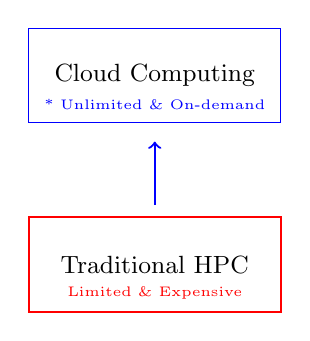
\begin{tikzpicture}[scale=0.8]
                % Traditional HPC box
                \draw[thick, red] (0,0) rectangle (4,1.5);
                \node at (2,0.75) {\small Traditional HPC};
                \node[red] at (2,0.3) {\tiny Limited \& Expensive};
                
                % Arrow
                \draw[->, thick, blue] (2, 1.7) -- (2, 2.7);
                
                % Cloud box
                \draw[blue] (0,3) rectangle (4,4.5);
                \node at (2,3.75) {\small Cloud Computing};
                \node[blue] at (2,3.3)  {\tiny * Unlimited \& On-demand};
            \end{tikzpicture}
        \end{column}
    \end{columns}
    
    \vspace{0.3cm}
    \begin{block}{The Opportunity}
        Cloud allows a better cost efficiency balance leveraging IaC, Devops and Data Interoperability
        
        \textbf{Vectorizing} here refers to transforming data into \textbf{embeddings}, not to loop vectorization (SIMD/GPU optimization in HPC)
    \end{block}
\end{frame}


% Slide 2: Scientific workflow
\begin{frame}{Scientific workflow}
    \begin{columns}
        \begin{column}{0.6\textwidth}
            \begin{itemize}
                \item A \textbf{data-centric} pipeline that transforms raw inputs into structured embeddings and feeds them into HPC simulations, with \textbf{iterative loop feedback} between \textbf{stages or phases} to boost performance and cost efficiency
                \item Generative AI for enhancing input dataset
                \item Data centric to ease workloads interoperability among different engine processing
                \item Embeddings to capture additional features and integrates with numeric simulation
            \end{itemize}
        \end{column}
        \begin{column}{0.4\textwidth}
            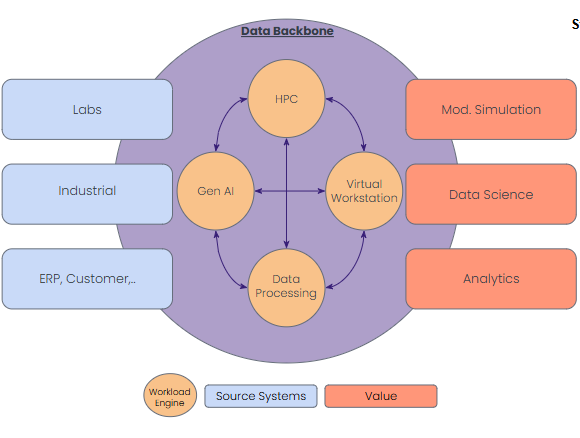
\includegraphics[width=\textwidth,height=0.6\textheight,keepaspectratio]{../../images/DataCentric-DataBackbone-Strategy.png}
        \end{column}
    \end{columns}
    
    \vspace{0.3cm}
    \begin{block}{Key Insight}
        \textbf {Tokens become embeddings} through learned matrix multiplication plus positional encoding via vector addition
    \end{block}
\end{frame}

% Slide 3: A Two-Phased
\begin{frame}{A Two-Phased Cloud-Native Architecture for Optimization}
    % Upper row with bullet points
    \begin{itemize}


\item \textbf{Scientific Workflow} Demands: Modern workloads need tech-stacks for high-throughput ETL, scalable HPC, distributed storage (S3/FSx), and heterogeneous compute (CPU/GPU/FPGA) to handle large, irregular datasets.

\item \textbf{Separation of Concerns}: A two-phase architecture cleanly decouples data preparation with Ray from numerical simulation with Slurm/MPI, ensuring modularity, scalability, and iterative feedback.

\item \textbf{Metagenomic Read Clustering}: Phase 1 converts FASTQ reads into LSHVec embeddings, stored as Parquet shards, which Phase 2 clusters in HPC jobs to identify microbial communities.

\item Pipeline Value: This design achieves \textbf{efficient handoff between ETL and HPC}, boosting reproducibility, performance, and cost-aware scaling in cloud environments.
        
    \end{itemize}
        
    \vspace{0.3cm}
    \begin{block}{Workload Example}
        \textbf{Metagenomics pipeline}  - FASTQ reads → k-mer embeddings → organism clustering
    \end{block}
\end{frame}


% Slide 3: A Two-Phased
\begin{frame}{A Two-Phased Cloud-Native Architecture for Optimization}
    % Upper row with bullet points
        \vspace{0.4cm}
    
    % Bottom row with image
    \begin{center}
        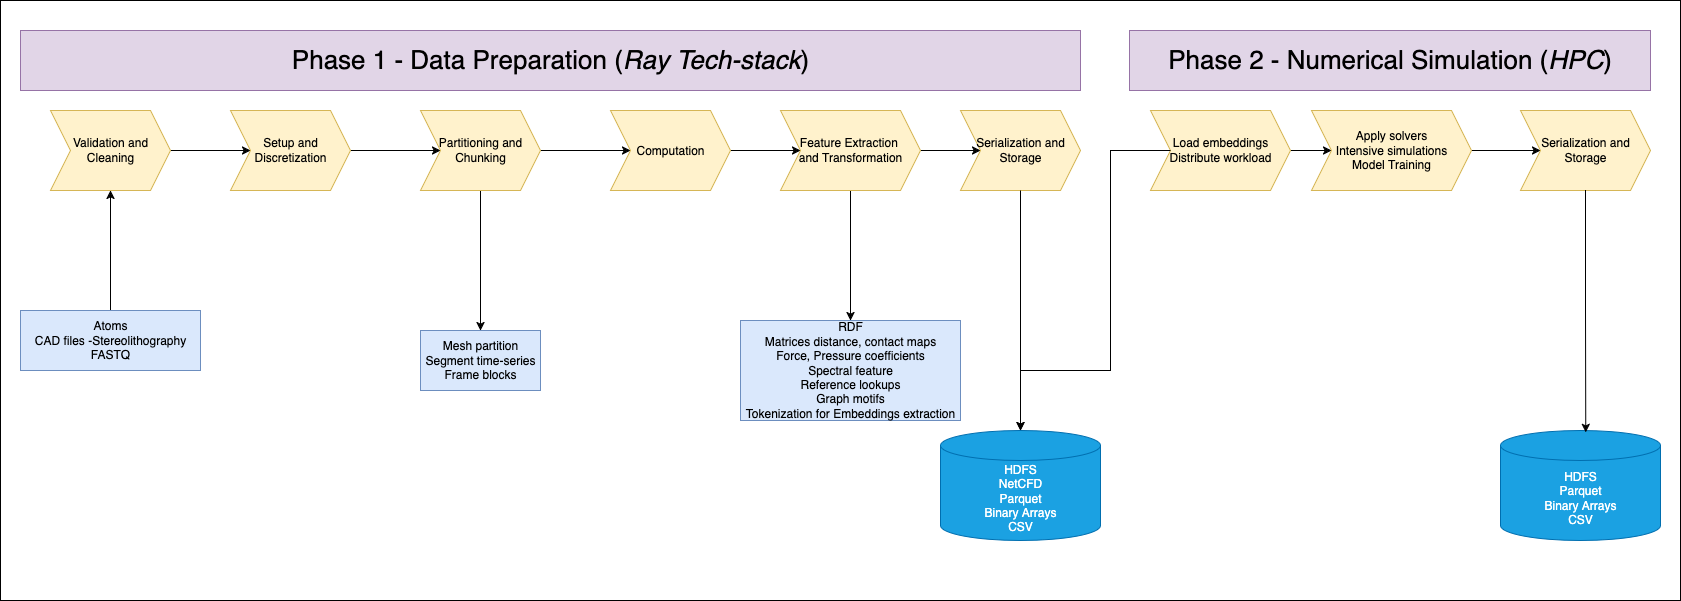
\includegraphics[width=1\textwidth,height=0.6\textheight,keepaspectratio]{../../images/Generalized_data-pipeline.drawio.png}
    \end{center}
        
    \vspace{0.3cm}
    \begin{block}{Workload Example}
        \textbf{Metagenomics pipeline}  - FASTQ reads → k-mer embeddings → organism clustering
    \end{block}
\end{frame}


% Slide 4: Two-Phased Architecture
\begin{frame}{A Two-Phased Cloud-Native Architecture for Optimization}
    % Push diagram up a bit to leave room for footnotes
    \vspace{-0.8cm}
    \begin{center}
        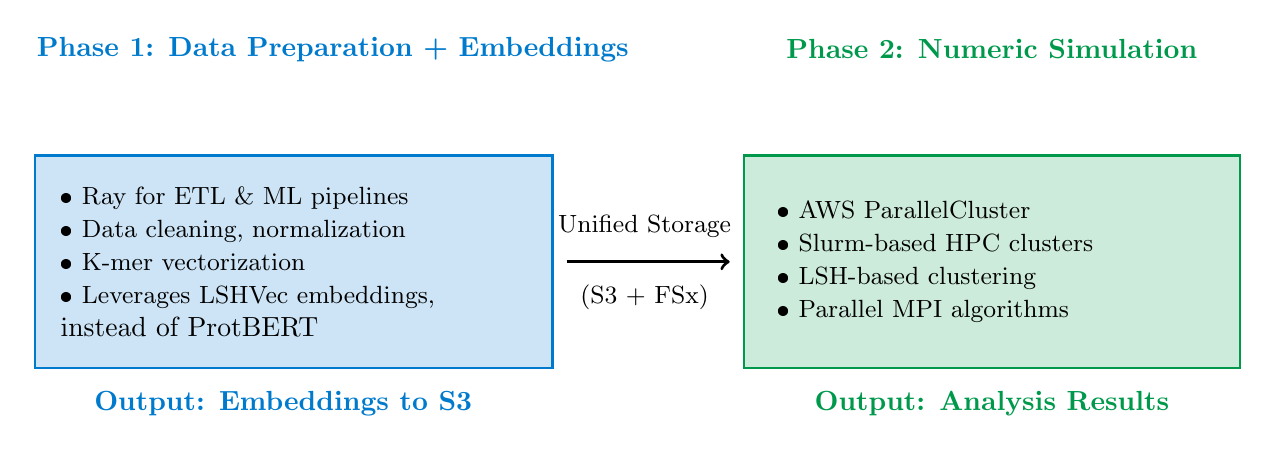
\begin{tikzpicture}[scale=0.9]
            % Phase 1 box
            \draw[thick, rayblue, fill=rayblue!20] (-3,0) rectangle (4.3,3);
            \node[rayblue, font=\bfseries] at (1.2,4.5) {Phase 1: Data Preparation + Embeddings};
            \node[align=left] at (0.0,1.5) {
                \small • Ray for ETL \& ML pipelines \\
                \small • Data cleaning, normalization \\
                \small • K-mer vectorization \\
                \small • Leverages LSHVec embeddings, \\ instead of ProtBERT
            };
            \node[rayblue] at (0.5,-0.5) {\textbf{Output: Embeddings to S3}};
            
            % Arrow
            \draw[->, very thick, black] (4.5, 1.5) -- (6.8, 1.5);
            \node at (5.6, 2) {\small Unified Storage};
            \node at (5.6, 1) {\small (S3 + FSx)};
            
            % Phase 2 box
            \draw[thick, hpcgreen, fill=hpcgreen!20] (7,0) rectangle (14,3);
            \node[hpcgreen, font=\bfseries] at (10.5,4.5) {Phase 2: Numeric Simulation};
            \node[align=left] at (9.7,1.5) {
                \small • AWS ParallelCluster \\
                \small • Slurm-based HPC clusters \\
                \small • LSH-based clustering \\
                \small • Parallel MPI algorithms
            };
            \node[hpcgreen] at (10.5,-0.5) {\textbf{Output: Analysis Results}};
        \end{tikzpicture}
    \end{center}
    
    % Reduce spacing after diagram to reclaim space
    \vspace{-0.4cm}
    \begin{block}{Key Integration}
        \textbf{Unified storage layer}: Seamless data flowing between stages and high-throughput access
        
        \textbf{To chain Phase 1 - Phase 2}: Event-driven workflow; Job Submit; pull-trigger-flag
    \end{block}
\end{frame}


% Slide 5: DNA Embedding Models for Ray Anyscale Deployment
\begin{frame}{DNA Embedding Models for Ray Anyscale Deployment}

\begin{itemize}
    \item \textbf{DNABERT-2:} SoTA accuracy, 322B+ DNA tokens, Ray HuggingFace integration
    \item \textbf{LSHVec:} Optimal scalability for terabyte-scale datasets with native distributed architecture and LSH optimization
    \item \textbf{fastDNA:} Fastest inference performance with lightweight k-mer embeddings
    \item \textbf{ProtBERT:} Protein-specific model incompatible with DNA sequences (amino acid vocabulary only)
\end{itemize}

\vfill

\begin{table}[b]
\centering
\tiny
\begin{tabular}{|p{2.2cm}|p{2.0cm}|p{2.0cm}|p{2.0cm}|p{2.0cm}|}
\hline
\textbf{Metric} & \textbf{DNABERT-2} & \textbf{LSHVec} & \textbf{fastDNA} & \textbf{ProtBERT} \\
\hline
\textbf{Primary Domain/ Training} & DNA (322B+ tokens) & DNA metagenomics & DNA metagenomics & Proteins (No DNA) \\
\hline
\textbf{Model Size} & 117M params & ~16M params & 10-100M params & 420M params \\
\hline
\textbf{Embedding Dimension} & 768 & 50-200 (config.) & 10-100 (config.) & 1024 \\
\hline
\textbf{Computation Optimization} & BPE + attention & LSH + skip-gram & k-mer embeddings & BERT masked LM \\
\hline
\textbf{Ray Fitness} & Excellent & Excellent & Good & Incompatible \\
\hline
\end{tabular}
\end{table}

    \vspace{0.3cm}
    \begin{block}{Tradeoff analysis}
        \textbf{Locality-Sensitive Hashing (LSH) Vec}: Designed for distributed training, to handle TB-scale datasets, hashing algorithm which dramatically reduces vocabulary size
    \end{block}

\end{frame}


% Slide 6: Phase 1
\begin{frame}{Phase 1 Deep Dive: Ray for Scalable Data Preprocessing}
    \begin{columns}
        \begin{column}{0.5\textwidth}
            \textbf{Ray's Role in Data Preparation:}
            \begin{itemize}
                \item \textbf{Data Ingestion:} Raw FASTQ reads processing as parquet files
                \item \textbf{K-mer Embeddings:} Using \textcolor{rayblue}{\textbf{LSHVec}} for fixed-length embeddings extraction
                \item \textbf{Parallel Processing:} Lightweight tasks across CPUs/GPUs
                \item \textbf{Output:} Parquet shards to Amazon S3 - FSxLustre
            \end{itemize}
        \end{column}
        \begin{column}{0.5\textwidth}
            \textbf{Performance \& Efficiency:}
            \begin{table}[h]
                \centering
                \small
                \begin{tabular}{lc}
                    \toprule
                    \textbf{Metric} & \textbf{Result} \\
                    \midrule
                    Scaling (1→2 GPUs) & (xx)× throughput \\
                    Processing rate & ~yy MB/s \\
                    Node startup time & ~xxs \\
                    Spot Instance savings & \textcolor{green}{\textbf{YY\%}} \\
                    Cost per GB & \textcolor{green}{\textbf{\$x.xx}} \\
                    \bottomrule
                \end{tabular}
            \end{table}
        \end{column}
    \end{columns}
    
    \vspace{0.3cm}
    \begin{block}{Key Achievement}
        \textbf{Fully automation} with Ray autoscaler dynamically managing cluster size and achieving operational and cost efficiency through Spot Instances
    \end{block}
\end{frame}

% Slide 7: Phase 2
\begin{frame}{Phase 2 Deep Dive: HPC ParallelCluster \& Overall Impact}

            \textbf{HPC Simulation with AWS ParallelCluster:}
            \begin{itemize}
                \item \textbf{Embedding Consumption:} Direct access from FSx/S3
                \item \textbf{Specialized Compute:} P4d instances with \textcolor{awsorange}{\textbf{NVIDIA A100 GPUs}}
                \item \textbf{Low-latency Communication:} Elastic Fabric Adapter (EFA) for MPI
                \item \textbf{Clustering Algorithms:} Parallel LSH and k-means for organism grouping
            \end{itemize}

    
    \vspace{0.3cm}
    \begin{block}{Synergistic Performance \& Benefits}
        \begin{itemize}
            
            \item \textbf{Extreme-scale Processing:} GPU acceleration for DNA sequencing processing performance
            \item \textbf{Developer Agility:} ParallelCluster automation for HPC cluster deployment
        \end{itemize}
    \end{block}
\end{frame}

% Slide 8: Conclusions
\begin{frame}{Conclusions}
    \begin{columns}
        \begin{column}{0.7\textwidth}
            \textbf{Key Conclusions:}
            \begin{itemize}
                \item \textbf{Iterative feedback loop} 
                \item Cloud Two-phase architecture delivers \textbf{significant gains} in elasticity, performance, interoperability and cost-efficiency
                \item Automated life-cycle management and Spot Instances ensure {\textbf{optimized resource utilization}}
                \item Successfully \textbf{decouples feature engineering from raw simulation workloads}
                
            \end{itemize}
        \end{column}
        \begin{column}{0.3\textwidth}
            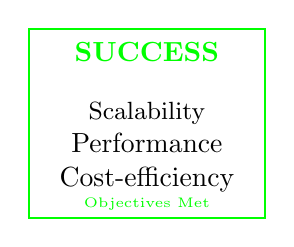
\begin{tikzpicture}[scale=0.6]
                % Success metrics visualization
                \draw[thick, green] (-1,0) -- (-1,4) -- (4,4) -- (4,0) -- cycle;
                \node[green, font=\bfseries] at (1.5,3.5) {SUCCESS};
                \node[align=center] at (1.5,1.5) {\small Scalability \\ Performance \\ Cost-efficiency};
                \node[green] at (1.5,0.3) {\tiny Objectives Met};
            \end{tikzpicture}
        \end{column}
    \end{columns}
    
    \vspace{0.3cm}
    \begin{block}{Key achievements}
        \begin{itemize}
            \item \textbf{Ray autoscaler (EC2 + GPU):} Maximize scalability for \textbf{DNA embedding extraction}
            \item \textbf{Storage at scale S3 FsxLustre:} Ease data interoperability
        \end{itemize}
    \end{block}
\end{frame}

% Slide 9: Future Directions
\begin{frame}{Future Directions}

            \textbf{Key Emerging Capabilities:}
            \begin{itemize}

                \item \textcolor{rayblue}{\textbf{GPU-accelerated Ray clusters highest scalability}} for DNA embedding extraction
                \item Evaluating Serverless ETL (AWS Glue) vs. Ray with GPU acceleration
                \item \textbf{Elastic Fabric Adapter} for low-latency + Amazon \textbf{FSx for Lustre} for high-throughput
            \end{itemize}

    
    \vspace{0.3cm}
    \begin{block}{Future Work \& Research Avenues}
        \begin{itemize}
            \item \textbf{FPGA Workloads:} Explore AWS F1 instances as alternative for accelerating the Smith-Waterman algorithm
            \item \textbf{Apple M-Series SoCs:} Metal Shading Language for chemical engineering or image classification/inference
            \item \textbf{Agentic AI for HPC already reality:} Microsoft Discovery - Workflow/Solver Agents; Data Centric + \textbf{Iterative feedback loop} across processing engines
            \item The investigations will continue, however, the data found so far confirm the initial hypothesis
        \end{itemize}
    \end{block}
\end{frame}

% Slide 10: The New Frontier
\begin{frame}{Studied Topics}
    \begin{center}
        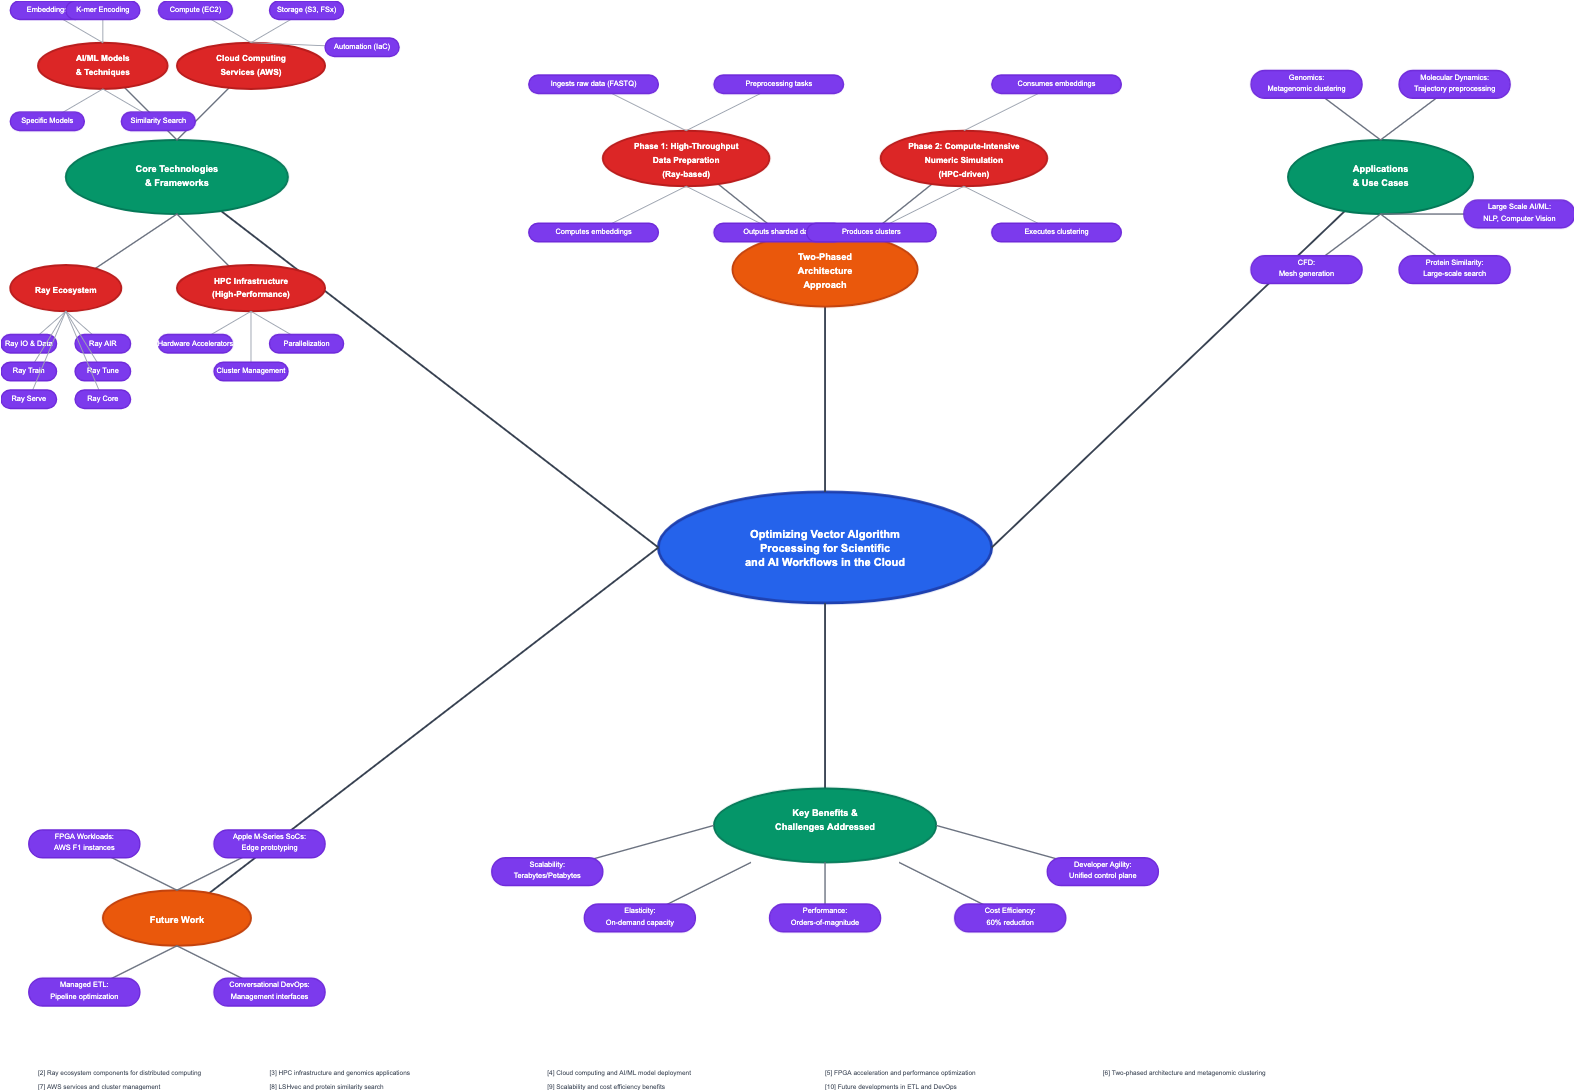
\includegraphics[width=0.9\textwidth,height=0.6\textheight,keepaspectratio]{../../images/TFM-MindMap.drawio.png}
    \end{center}
    
    \vspace{0.3cm}
    \begin{block}{Centric idea}
        \textbf{Optimizing Vector Algorithm - Embeddings extraction}:  Processing through the integration of Ray IO and HPC in the Cloud
    \end{block}
\end{frame}

% Thank you slide
\begin{frame}[plain]
    \begin{center}
        \Huge Thank You!
        
        \vspace{1cm}
        \Large Questions?
        
        \vspace{0.8cm}
        \normalsize
        \textbf{Optimizing Vector Algorithm Processing through the integration of Ray IO and HPC in the Cloud}
        
        \vspace{0.5cm}
        Tiago de Souza de Oliveira \\
        \texttt{tiago.souza@rai.usc.es, tiagoooliveira@qmind-lab.com}
    \end{center}
\end{frame}

\end{document}